\section{Results}
\label{s:results}
%Results; this should be a readable summary of the results from applying the approach. Don’t pursue death by figures but carefully select what visualisations (figures, tables) are functional for telling your story and logically lead to the main conclusions and policy advice?

% Convincing story, consistent with approach using carefully designed visuals and tables to support narrative
In this section, we summarise the key results from applying this approach, first identifying the most robust policies for Gorssel, Deventer and Overijssel, and subsequently discussing options for synthesising policy choices between the three actors. 

\subsection{Robust Decision Making}
%Look at the policies for the five different scenarios, and examine trade-offs using different robustness metrics.
For the robust decision making process two metrics were used: Satisficing (the domain-criterion) and maximum regret. 
%#################################################################
%   REGRET AND SATISFICING - GORSSEL
%#################################################################
\subsubsection{Gorssel}
The results for Gorssel's satisficing analysis with the domain criterion are shown in \autoref{fig:domain_criterion_gorssel}. The twelve selected policies are analysed for trade-offs and the extent to which the results satisfy Gorssel's threshold values. \newline
\autoref{fig:domain_criterion_gorssel} shows that every policy is satisficing for "Gorssel Expected Number of Deaths". This means that all potential policy recommendations ensure that the legal standards for citizen safety are met in all tested scenarios. 
It can also be observed that Gorssel's G\_1 policy performs best for the domain-criterion results, reaching the highest domain-criterion scores on average. However, this policy comes with a big trade-off with the expected annual damage as the policy often goes over the annual damage budget, and thus reaches a low domain-criterion value for 'expected annual damage'. This would make the policy less robust in terms of damage and more in terms of costs. For the other policies it is the other way around. Most policies except for G\_1 score 0 on 'total costs' and these policies are thus not robust, when considering these satisficing results.  \newline

\noindent In \autoref{fig:regret_gorssel}, the results for Gorssel's regret analysis are shown. The least regret for Gorssel appears with policy G\_2. This is due to the fact that the expected number of Deaths and the Damage for Gorssel have 0 regret in this policy, this comes at a high total cost. This is a clear example of the trade-offs that have to be made within the policies. A trade off like this is also shown with policy G\_8, where there is little regret for the damage but the number of deaths and the costs lead to high regret.

Another noteworthy result is that some of the policies that have a high regret, have a low satisficing score, and vice-versa.

\begin{figure}[H]
  \centering
  \begin{minipage}[b]{0.4\textwidth}
    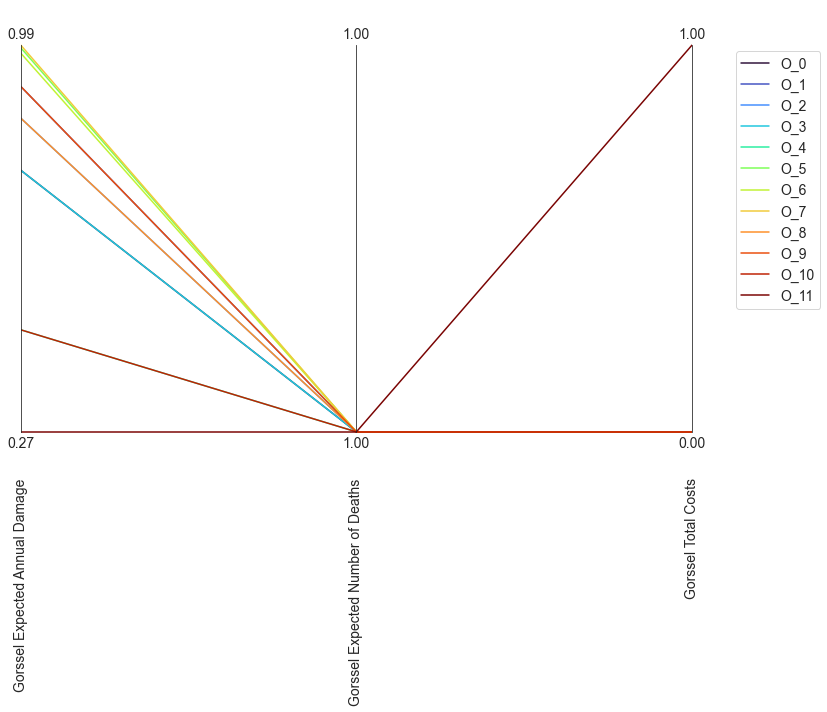
\includegraphics[width=1.15\textwidth]{report/figures/results/domain_criterion_Gorssel.png}
    \caption{Results for Gorssel's domain criterion}
    \label{fig:domain_criterion_gorssel}
  \end{minipage}
  \hfill
  \begin{minipage}[b]{0.4\textwidth}
    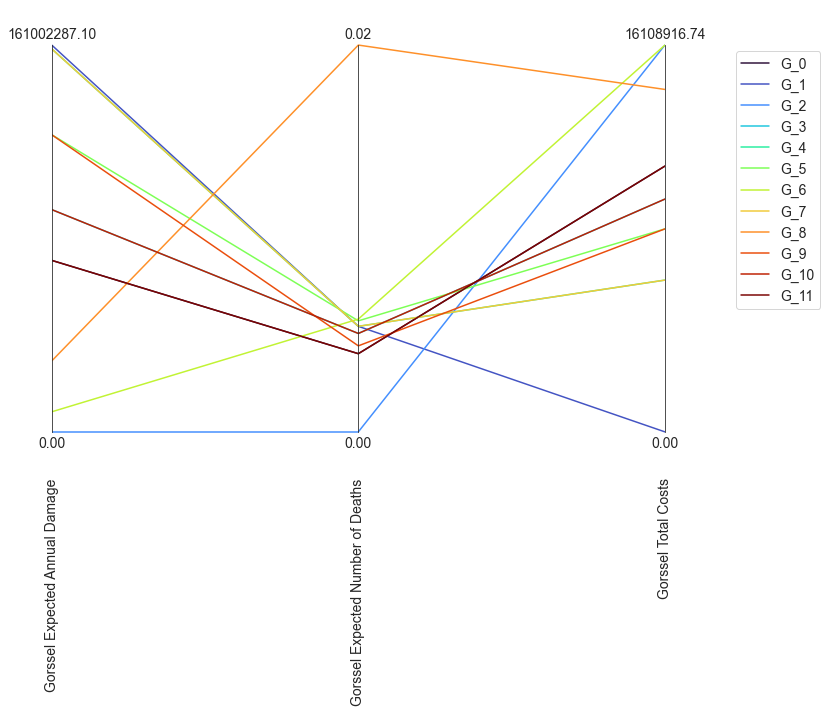
\includegraphics[width=1.15\textwidth]{report/figures/results/regret_figure_Gorssel.png}
    \caption{Results for Gorssel's maximum regret}
    \label{fig:regret_gorssel}
  \end{minipage}
\end{figure}




%#################################################################
%   REGRET AND SATISFICING - DEVENTER
%#################################################################
\subsubsection{Deventer}
The results for Deventer's satisficing analysis with the domain criterion are shown in  \autoref{fig:domain_criterion_Deventers}. 
\autoref{fig:domain_criterion_Deventers} shows that every policy is satisficing for "Deventer Expected Number of Deaths" and for "Deventer Total Costs". This means that later policy recommendations, just like in Gorssel's case, are ensured that the legal standards for citizen safety will be met in all scenarios and that the budget of Deventer never overextends (within the set thresholds). 

The policy G\_9 together with D\_8 performed the best with the satisficing scores for the expected damage. The other policies score only a little over half of this value. As such, policy D\_8 and D\_9 are the more robust policies. \newline 

\noindent \autoref{fig:regret_Deventers} shows the regret results for Deventer's policy options. Here it can be seen that policy D\_8 and D\_9 score the best on the 'average' regret with certain trade-offs. Especially policy D\_9 shows a big trade-off compared to D\_8 between expected damage and expected deaths versus the total costs that this brings with it. Another policy that reveals potential policy strategies for Deventer is policy D\_4. This policy shows that only way Deventer will not 'regret' their total costs is when they trade costs for high damages and high expected number of deaths. 
\begin{figure}[H]
  \centering
  \begin{minipage}[b]{0.4\textwidth}
    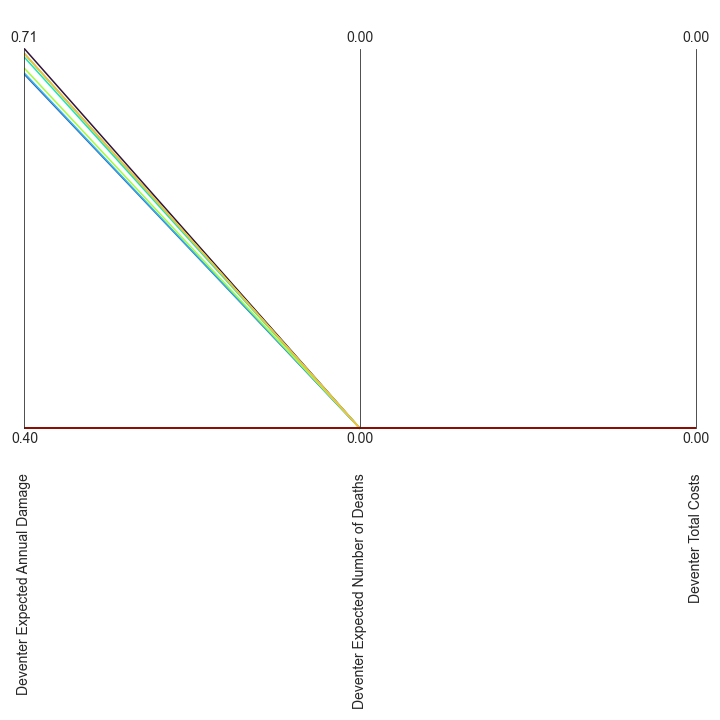
\includegraphics[width=1.2\textwidth]{report/figures/results/domain_criterion_Deventer.png}
    \caption{Results for Deventer's domain criterion}
    \label{fig:domain_criterion_Deventers}
  \end{minipage}
  \hfill
  \begin{minipage}[b]{0.4\textwidth}
    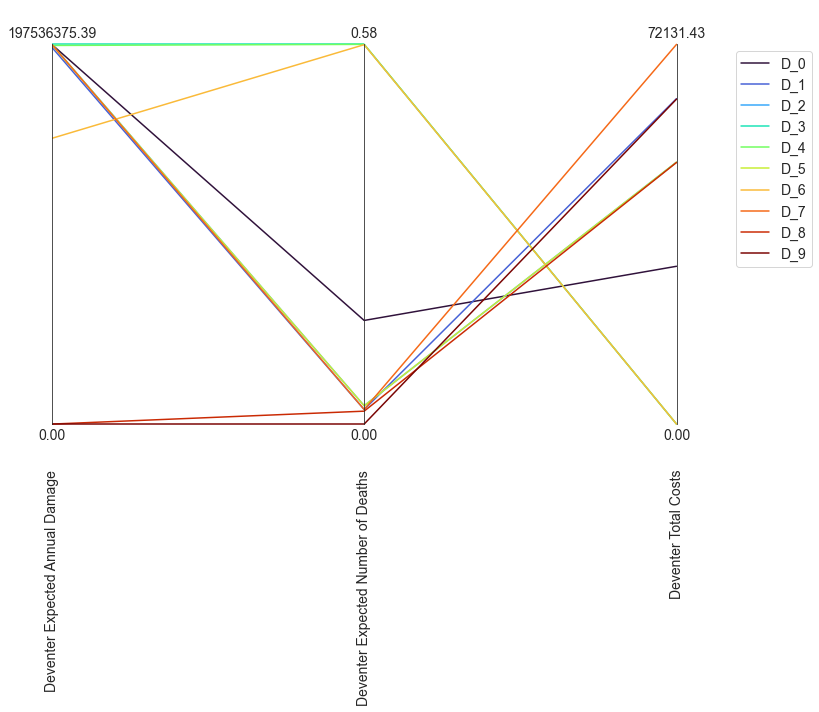
\includegraphics[width=1.2\textwidth]{report/figures/results/regret_figure_Deventer.png}
    \caption{Results for Deventer's maximum regret}
    \label{fig:regret_Deventers}
  \end{minipage}
\end{figure}

%#################################################################
%   REGRET AND SATISFICING - OVERIJSSEL
%#################################################################
\subsubsection{Overijssel}
Overijssel's satisficing analysis with the domain criterion are shown in \autoref{fig:domain_criterion_Overijssels}. It can be seen that every policy is satisficing for "Gorssel and Deventer Expected Number of Deaths" and none with the exception of O\_6 for "Gorssel and Deventer Total Costs". And thus, all potential policy recommendations can be sure that the legal standards for citizen safety will be met in all scenarios while crossing the total cost threshold of Overijssel, except for O\_6 because it does not satisfice for costs. 
Policy O\_8 and policy O\_10 are one of the better choices, scoring low on regret based on their satisficing scores due to their scores on 'expected damage'. \newline

\noindent \autoref{fig:domain_criterion_Overijssels} shows the regret results for Overijssel's policy options. Here policy O\_8 and O\_10 score the best on the 'average' regret, but due show certain trade-offs. It is interesting to note that policy D\_10 shows almost no trade-off compared to the other policies.

\begin{figure}[H]
  \centering
  \begin{minipage}[b]{0.4\textwidth}
    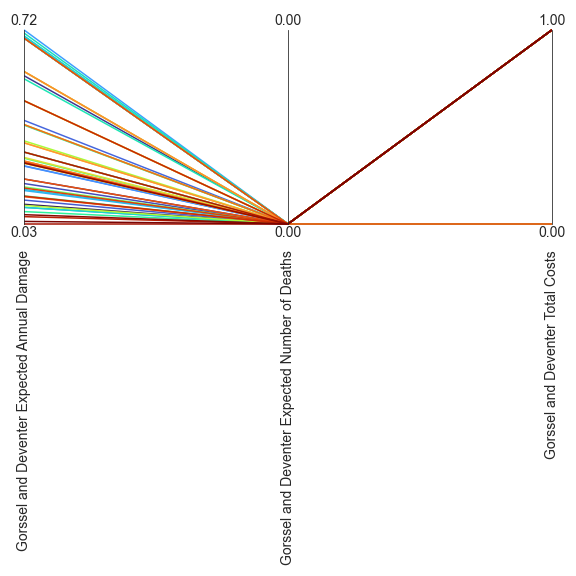
\includegraphics[width=1.2\textwidth]{report/figures/results/domain_criterion_Overijssel.png}
    \caption{Results for Overijssel's domain criterion}
    \label{fig:domain_criterion_Overijssels}
  \end{minipage}
  \hfill
  \begin{minipage}[b]{0.4\textwidth}
    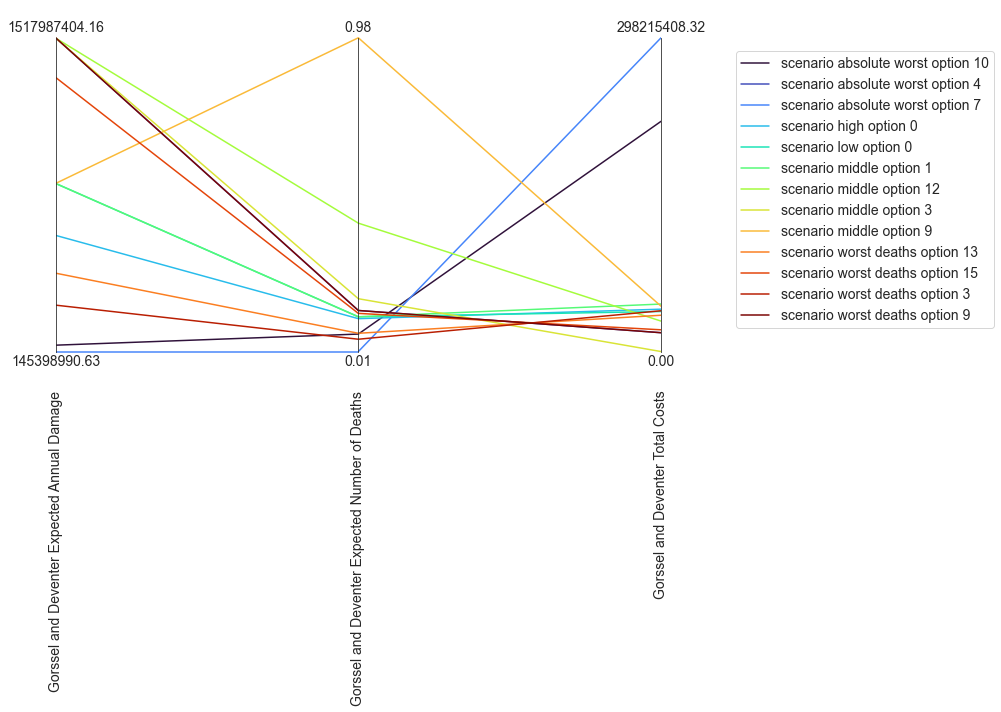
\includegraphics[width=1.2\textwidth]{report/figures/results/regret_figure_Overijssel.png}
    \caption{Results for Overijssel's maximum regret}
    \label{fig:regret_Overijssels}
  \end{minipage}
\end{figure}


\subsection{Sensitivity Analysis}

To see which uncertainties and levers have a large effect on model behaviour, a sensitivity analysis was carried out as explained in \autoref{ss:sensitivity-analysis}. The analysis of these can be viewed per actor in the following section. The generated figures for the sensitivity analysis can be found in \autoref{a:sensitivity-analysis}.

%Firstly, the sensitivity analysis was done with feature scoring without the policies to get a grasp of which uncertainty and levers the actors would be most sensitive to. After, policies are added and analysed to assess whether they would be sensitive or not. 

\subsubsection{Gorssel}

From the sensitivity analysis for damage and deaths for Gorssel it becomes apparent that they are not only influenced by their own dike durability, but also by that of Deventer. As a result, the failures of \textit{both} cities have the highest impact on the deaths and damage. When adding the policies, we observe that the sensitivity to dike durability remains the highest for both the deaths and damage. 

\subsubsection{Deventer}

For Deventer the biggest threat to damages and deaths is the dike durability of just Deventer. This is in line with expectations, because only their own dikes breaking would impact Deventer. And just as with Gorssel, we can observe that when adding the policies, we see that the outcome is still least robust under dike failure. 

\subsubsection{Overijssel}

For the costs of the province of Overijssel it can be observed that they are sensitive to dike increase. The sensitivity is biggest to dike increase in Gorssel, which is in line with reality as this is the most costly procedure in the province, other than Room for the River. However, because none of the policies for Overijssel recommend Room for the River, there is no observed sensitivity. Furthermore, the entire province shows a higher score on deaths and damages across the province as well when it comes to dike failure. 

\subsection{Shortlisted Policies per Actor}
From the robustness analysis, a subset of the top five most robust policies (prioritising regret-based metrics) were identified. Here, a brief summary of each policy in terms of dike heightening, Room the the River projects, and early warning systems are presented for each actor. The damage, death, and cost outcomes are not included in these tables, as they are already assumed to have been optimised to be within acceptable levels based on the robustness metrics in previous steps. Policies were qualitatively interpreted for opportunities for coalition forming, with relevant policies highlighted yellow in each table.

Interpreting these policies for opportunities for coalition-forming, there is a commonly re-occurring objective of a three-day early warning, which presents an opening for consensus-building between actors in the Overijssel region. The tables below explore this in more detail.

\subsubsection{Gorssel}
The five most robust policies for Gorssel are presented in Table \ref{tab:gpols}

\begin{table}[h!]
  \centering
  \captionsetup{justification=centering,margin=2cm}
  \caption{Robust policies for Gorssel. RfR stands for Room for the River, dike increases are in decimetres and aggregated over all planning steps, EWS refers to Early Warning System in days}
  \label{tab:gpols}
  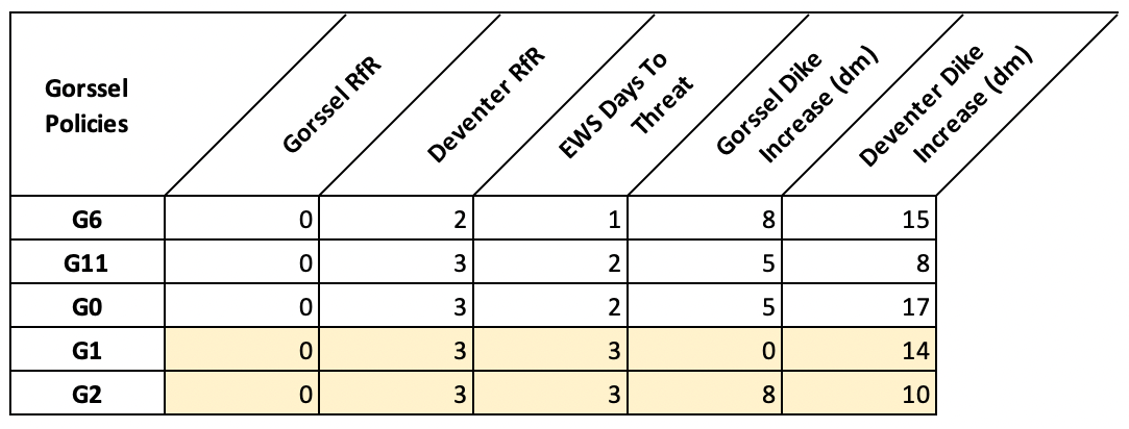
\includegraphics[width=0.8\linewidth]{report/figures/gpols.png}
\end{table}

\noindent Obviously, given that these policies are optimised for Gorssel's objectives, all of these policies are favourable for Gorssel. However, we highlight policies G1 and G2 for opportunities they present for coalition forming with Deventer and Overijssel. Arguably, these two policies are less favourable for Deventer, given the larger investments in Room for the River and dike increases. However, they are well-aligned with many of Overijssel's preferred policies (seen in Table \ref{tab:opols}) which prioritise earlier warnings and modest dike heightening (although they do not include Room for the River policies).

\subsubsection{Deventer}
The five most robust policies for Deventer are presented in Table \ref{tab:dpols}

\begin{table}[h!]
  \centering
  \captionsetup{justification=centering,margin=2cm}
  \caption{Robust policies for Deventer. RfR stands for Room for the River, dike increases are in decimetres and aggregated over all planning steps, EWS refers to Early Warning System in days}
  \label{tab:dpols}
  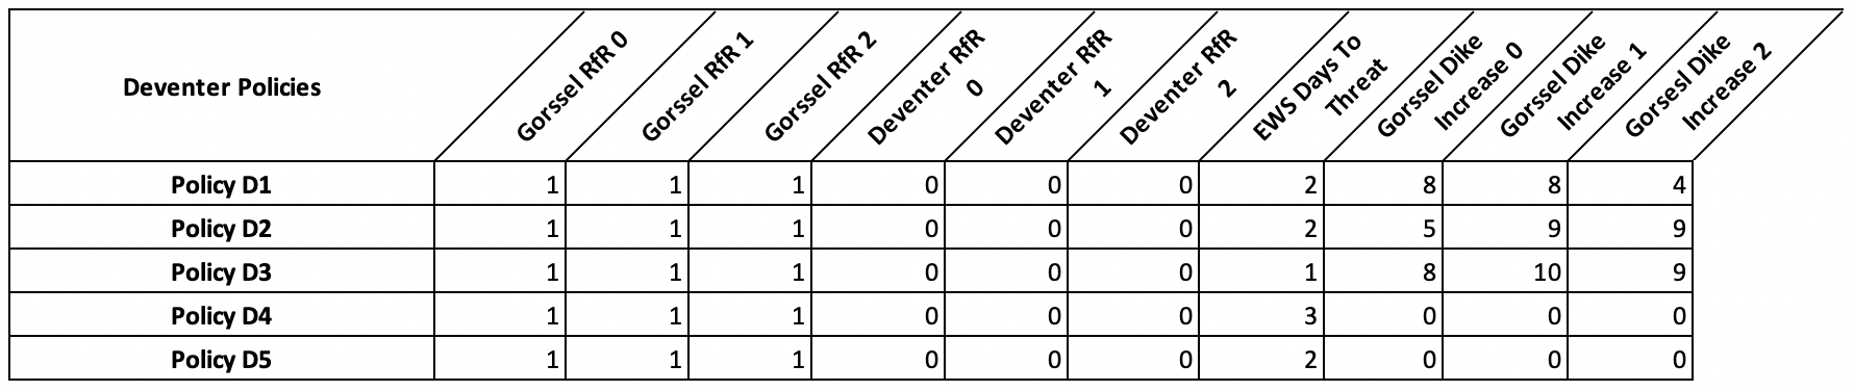
\includegraphics[width=0.8\linewidth]{report/figures/dpols.png}
\end{table}

Deventer's policies offer the least to Gorssel in terms of potential coalition-forming/points for negotiation. Of interest, however, is policy D9. This policy, while requiring significant Room for the River investment in Gorssel, does not require any dike heightening (as for all other robust policies for Deventer), relying instead on earlier warnings, similar to related robust policies of Gorssel and Overijssel.

\subsubsection{Overijssel}
The five most robust policies for Overijssel are presented in Table \ref{tab:opols}

\begin{table}[h!]
  \centering
  \captionsetup{justification=centering,margin=2cm}
  \caption{Robust policies for Overijssel. RfR stands for Room for the River, dike increases are in decimetres and aggregated over all planning steps, EWS refers to Early Warning System}
  \label{tab:opols}
  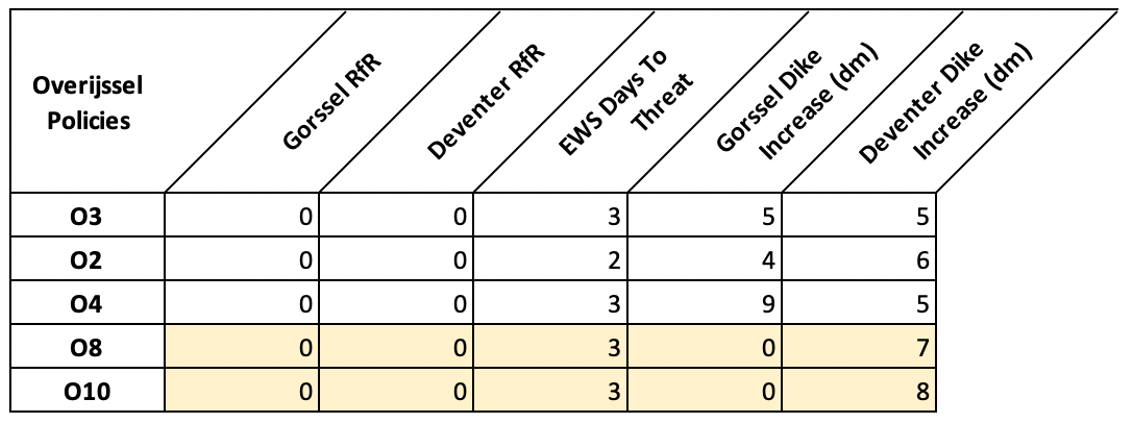
\includegraphics[width=0.8\linewidth]{report/figures/opols.png}
\end{table}

\noindent Overijssel's policies prioritise dike increases in the first planning step, with none of the policies prioritising Room for the River (reflecting the relative expense of these policies compared to dike increases). Of interest to Gorssel is policies O8 and O10 (highlighted yellow in the table). These two policies are favourable for both Gorssel and Overijssel (given minimal investment costs in Gorssel), and present an opportunity for starting discussions with Overijssel Province for pursuing such a policy.

\subsection{Policy Comparison}
Here, the top five policies from Deventer and Overijssel are considered and compared in terms of their performance against Gorssel's key outcomes.

\begin{figure}[h!]
    \centering
    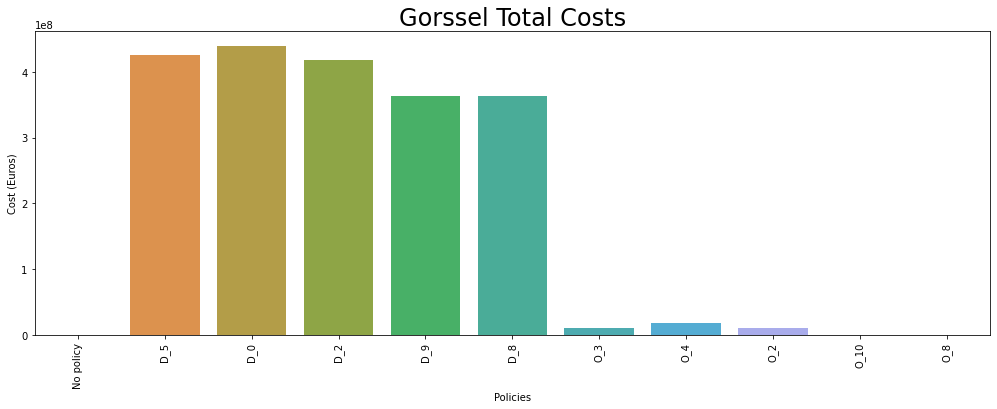
\includegraphics[width=\textwidth]{report/figures/results/spreads/cost_policies_Gorssel.png}
    \caption{Costs to Gorssel for Deventer's and Overijssel's top five most robust policies}
    \label{fig:cost-pol-g}
\end{figure}

\begin{figure}[h!]
    \centering
    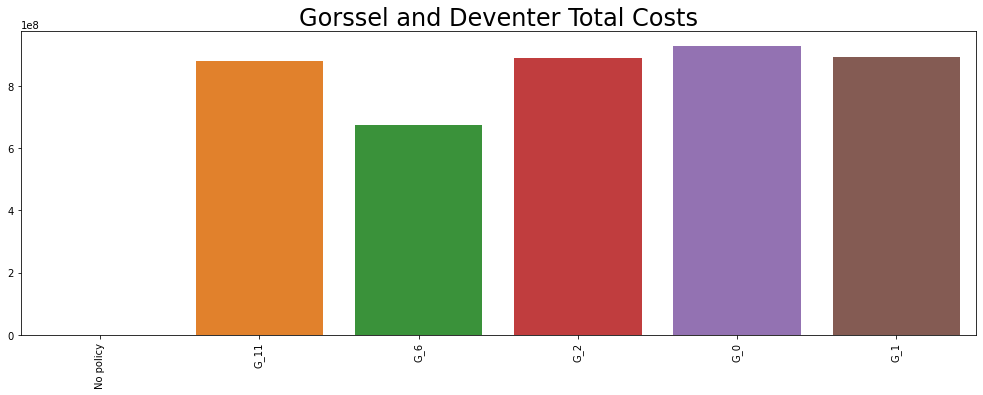
\includegraphics[width=\textwidth]{report/figures/results/spreads/cost_policies_Overijssel.png}
    \caption{Costs of Overijssel's top five most robust policies}
    \label{fig:cost-pol-o}
\end{figure}

\subsection{Summary of Policy Recommendations}
Based on the above results, there are four key pieces of policy advice for the Municipality of Gorssel:
\begin{itemize}
    \item Modest dike increases in both Gorssel and Deventer in the first planning step present a robust solution to minimise flood risk in Gorssel.
    \item Gorssel should support or initiate the Overijsssel regional government in lobbying for an increase of the Early Warning System to 3 days.
    \item The current scoping of the problem suggests that Room for the River projects are not favourable due to relative costs (compared to dike increases). However, the sensitivity of proposed policies to uncertainty in the probability of a dike failure suggests that these options may warrant further exploration as a policy option.
    \item We recommend - should Gorssel pursue dike heightening projects and EWS increases - that they complement these policies with other activities to improve their real-world robustness. For example, instantiating improved monitoring and evaluation of dike strength to proactively minimise uncertainty and risk, and/or public relations/community engagement strategies to improve the uptake and acceptance of the increased (and potentially more frequent) warnings.
\end{itemize}